% Auto-generated by 04_additional_analysis.R — do not edit
% y > 0: Overreacts  |  y < 0: Underreacts
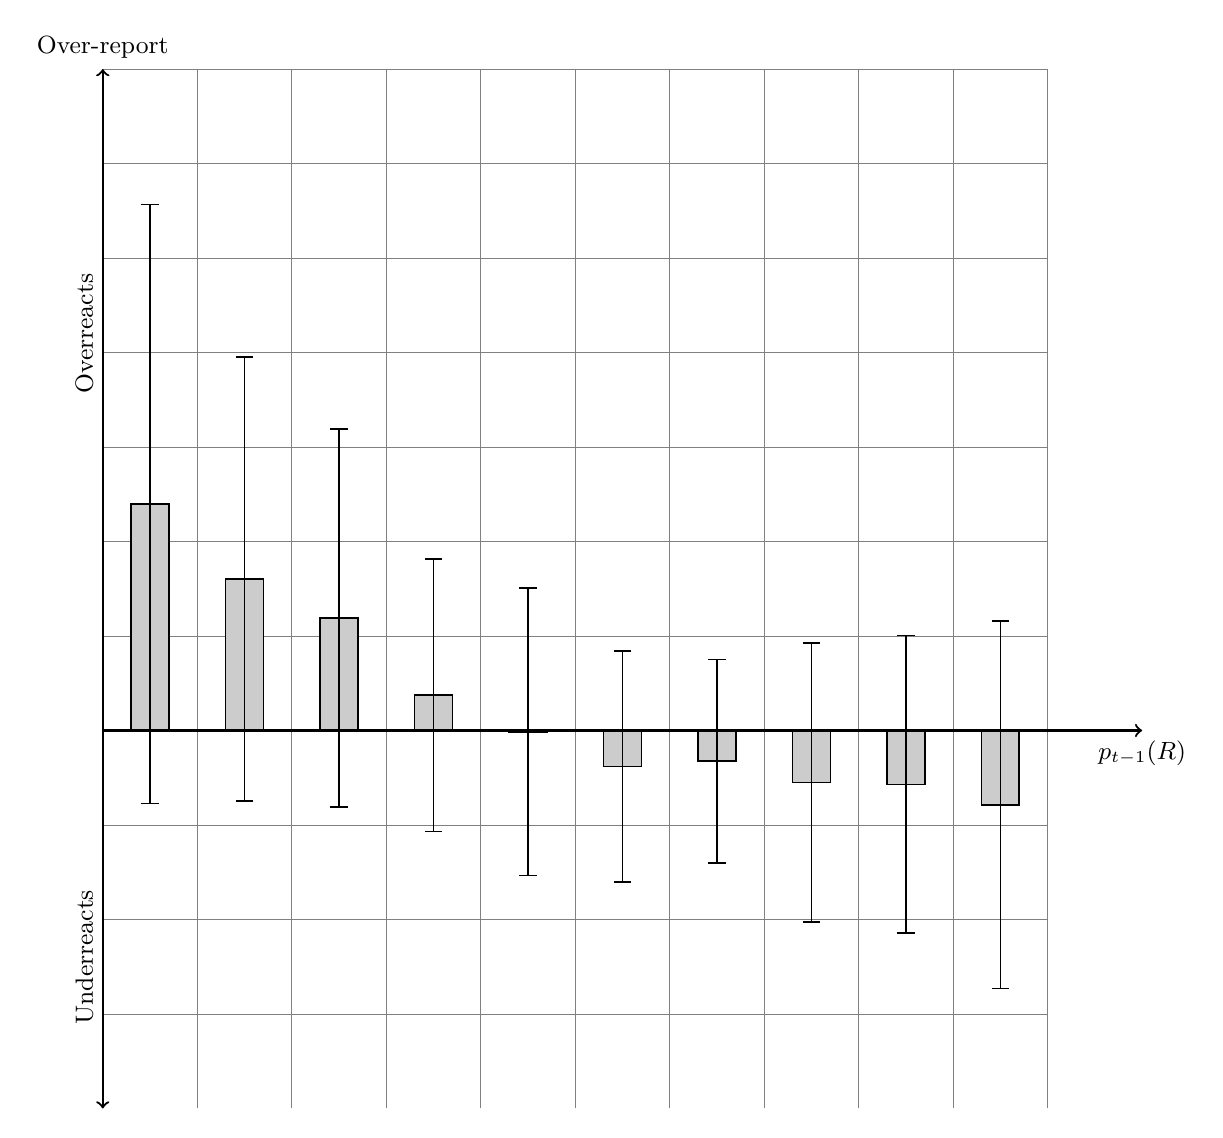
\begin{tikzpicture}[scale=12]
\draw[help lines,step=0.1] (0,-0.4) grid (1,0.7);
\filldraw[opaque,white!80!black] (0.03,0) rectangle (0.07,0.2396);
\draw[line width=0.6] (0.03,0) rectangle (0.07,0.2396);
\draw[line width=0.6,|-|] (0.05,-0.0783) -- (0.05,0.5574);
\filldraw[opaque,white!80!black] (0.13,0) rectangle (0.17,0.1604);
\draw[line width=0.6] (0.13,0) rectangle (0.17,0.1604);
\draw[line width=0.6,|-|] (0.15,-0.0754) -- (0.15,0.3962);
\filldraw[opaque,white!80!black] (0.23,0) rectangle (0.27,0.1191);
\draw[line width=0.6] (0.23,0) rectangle (0.27,0.1191);
\draw[line width=0.6,|-|] (0.25,-0.0817) -- (0.25,0.3199);
\filldraw[opaque,white!80!black] (0.33,0) rectangle (0.37,0.0373);
\draw[line width=0.6] (0.33,0) rectangle (0.37,0.0373);
\draw[line width=0.6,|-|] (0.35,-0.1078) -- (0.35,0.1824);
\filldraw[opaque,white!80!black] (0.43,0) rectangle (0.47,-0.0014);
\draw[line width=0.6] (0.43,0) rectangle (0.47,-0.0014);
\draw[line width=0.6,|-|] (0.45,-0.1544) -- (0.45,0.1517);
\filldraw[opaque,white!80!black] (0.53,0) rectangle (0.57,-0.0382);
\draw[line width=0.6] (0.53,0) rectangle (0.57,-0.0382);
\draw[line width=0.6,|-|] (0.55,-0.1614) -- (0.55,0.0851);
\filldraw[opaque,white!80!black] (0.63,0) rectangle (0.67,-0.0324);
\draw[line width=0.6] (0.63,0) rectangle (0.67,-0.0324);
\draw[line width=0.6,|-|] (0.65,-0.1408) -- (0.65,0.0759);
\filldraw[opaque,white!80!black] (0.73,0) rectangle (0.77,-0.0550);
\draw[line width=0.6] (0.73,0) rectangle (0.77,-0.0550);
\draw[line width=0.6,|-|] (0.75,-0.2037) -- (0.75,0.0937);
\filldraw[opaque,white!80!black] (0.83,0) rectangle (0.87,-0.0570);
\draw[line width=0.6] (0.83,0) rectangle (0.87,-0.0570);
\draw[line width=0.6,|-|] (0.85,-0.2155) -- (0.85,0.1016);
\filldraw[opaque,white!80!black] (0.93,0) rectangle (0.97,-0.0787);
\draw[line width=0.6] (0.93,0) rectangle (0.97,-0.0787);
\draw[line width=0.6,|-|] (0.95,-0.2741) -- (0.95,0.1166);
\draw[line width=0.8,->]  (0,0) -- (1.1,0) node[below] {\small{$p_{t-1}(R)$}};
\draw[line width=0.8,<->] (0,-0.4) -- (0,0.7) node[above] {\small{Over-report}};
\draw (0,0.42) node[above,rotate=90] {\small{Overreacts}};
\draw (0,-0.24) node[above,rotate=90] {\small{Underreacts}};
% ADD THEORY CURVE BELOW IF NEEDED:
% \draw[red,line width=1.2,domain=0.01:0.99] plot(\x,{...});
\end{tikzpicture}
